% !TeX root = report.tex
% !TeX spellcheck = en_GB

\section{Experiment}
Given an unweighted undirected graph $G$, a source vertex $s$, and a target vertex $t$, find the shortest path from $s$ to $t$ in $G$.

\newpar We have restricted the problem to instances where a path between $s$ and $t$ exists.

\subsection{Instance encoding}
In order to feed the instance into the network, we use a one hot encoding of the adjacency matrix of the graph and each of the source and target vertices. See \autoref{fig:input:encoding} for an example.

\begin{figure}[ht]
	\centering
	\begin{subfigure}{.5\textwidth}
		\centering
		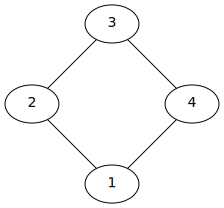
\includegraphics[width=\textwidth]{figures/encoding.png}
		\subcaption{}
	\end{subfigure}%
	\begin{subfigure}{.5\textwidth}
		\centering
		\begin{tabular}{|c|c|c|c|c|}
			\hline
			&\textbf{1}&\textbf{2}&\textbf{3}&\textbf{4}\\\hline
			\textbf{1}&0&1&0&0\\\hline
			\textbf{2}&1&0&1&1\\\hline
			\textbf{3}&0&1&0&1\\\hline
			\textbf{4}&0&1&1&0\\\hline
		\end{tabular}
		\subcaption{}
	\end{subfigure}\par\bigskip
	\begin{adjustbox}{center}
		\begin{subfigure}{1.3\textwidth}
			\centering
			\begin{tabu}{|c|c|c|c||c|c|c|c||c|c|c|c||c|c|c|c|[2pt]c|c|c|c|[2pt]c|c|c|c|}
				\hline
				0&1&0&0&1&0&1&1&0&1&0&1&0&1&1&0&1&0&0&0&0&0&0&1\\\hline
			\end{tabu}
			\subcaption{}
		\end{subfigure}
	\end{adjustbox}
	\caption{Shows a simple graph (a), its adjancency matrix (b) and an encoding where $s=1$ and $t=4$ (c). Thick lines between cells means encoding of a new structure. The three structures are the flattened adjacency table, with each row delimited with double lines for visibility, the one-hot encoding of $s$, and the one-hot encoding of $t$}
	\label{fig:input:encoding}
\end{figure}

\noindent When the neural network using the turing machine returns output, this is a one-hot encoding of the next vertex on the path to the target. Furthermore, for simplicity we choose the first node with maximal weight.

\newpar This means that we can run the graph through the neural network multiple times, and each time, the neural network will tell us which vertex to move to, which we can give it back as the new source vertex to move from.

\subsection{Instance generation}
Each experiment has a few settings that can be chosen between.
A number of these settings are related to instance generation.

\newpar We have made a factory that produces graphs containing a path of a specified length, but with the rest of the vertices connected to this path, in some fashion.

\newpar The configurations that can be chosen between for this factory is the following:

\begin{itemize}
	\item The number of vertices of the graph
	\item The length of the path that should be found in the graph
	\item The seed of the random number generator that is used to produce instances
	\item Whether or not the same graph should be used in symmetric instances, that is, one instance with a source and goal and another where they have been switched.
\end{itemize}

\noindent The factory then chooses a source and a goal, and builds a path of the specified length between them.
If there are any unused vertices left in the graph, they will become adjacent to some other vertex in the connected component of the path.
The last part is implemented to try to confuse the neural networks, since the input is given to them as an adjacency matrix.

\subsection{Fitness}
We have chosen to give the following scores for the output of each step on the shortest path:

\begin{itemize}
	\item[1] if there is an edge from the current vertex to the chosen vertex, but the distance from the chosen vertex to the goal vertex is greater than from the current vertex to the goal vertex.
	\item[2] if there is an edge from the current vertex to the chosen vertex, but the distance from the chosen vertex to the goal vertex is the same as from the current vertex to the goal vertex.
	\item[4] if there is an edge from the current vertex to the chosen vertex, but the distance from the chosen vertex to the goal vertex is less than from the current vertex to the goal vertex.
\end{itemize}

\noindent Furthermore, we give the score 0, if one step resulted in a move where no edge exists. Also the accumulated score is reset to 0, and no further steps are performed.

\newpar The idea behind these scores is that we want to reward neural networks that understand the underlying graph problem (or can at least guess them) more than a network that chooses arbitrarily.

\subsection{The Experiments}
To assess and measure how well the shortest path problem is solved, two times three experiments are performed. The first three experiments uses the NEAT framework to train and build the neural networks. The last three experiments uses the ENTM extension of the NEAT framework and can therefore in addition approximate Neural Turing machines. The memory is unlimited (within the bounds of the host machine), the write vector size is 4 and the default jump mechanism introduced in \cite{greve2016evolving} is used. 

\newpar Both networks uses the exact same configuration for NEAT and the general problem to make it easier to compare the two. Each configuration uses 30 species with population of 500. Each genome is tested on 25 unique graphs per generation. The entire configuration can be seen in appendix \todo{appendix}. 